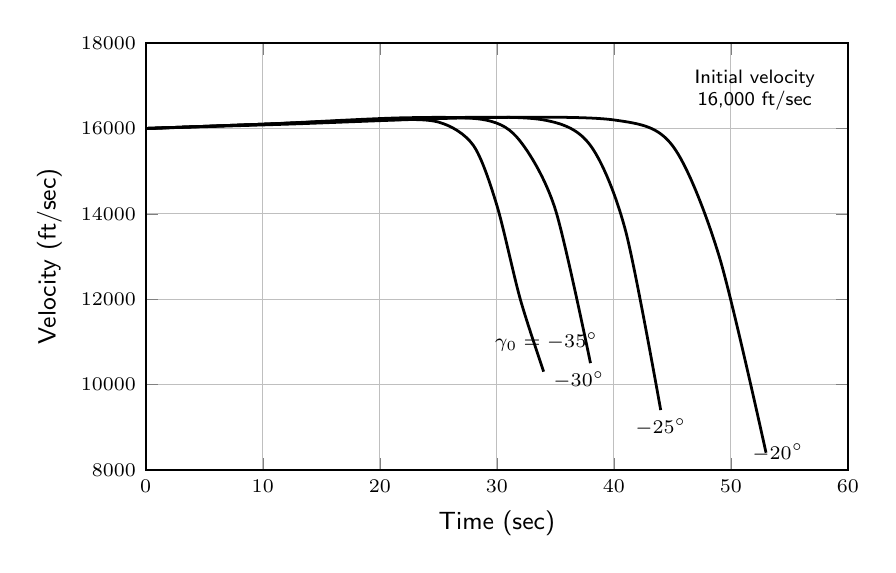
\begin{tikzpicture}
\begin{axis}[
  width=10.5cm,height=7.0cm,
  xmin=0,xmax=60,ymin=8000,ymax=18000,
  xtick={0,10,20,30,40,50,60},
  ytick={8000,10000,12000,14000,16000,18000},
  grid=major,
  axis line style={line width=0.8pt},
  tick label style={font=\scriptsize},
  label style={font=\sffamily\small},
  xlabel={Time (sec)},ylabel={Velocity (ft/sec)},
  scaled y ticks=false,
  yticklabel style={/pgf/number format/fixed,/pgf/number format/1000 sep={}},
]
  \addplot[line width=1.0pt,smooth] coordinates {(0,16000) (10,16100) (20,16200) (25,16150) (28,15600) (30,14200) (32,12000) (34,10300)};
  \addplot[line width=1.0pt,smooth] coordinates {(0,16000) (10,16100) (22,16250) (29,16200) (32,15700) (35,14100) (38,10500)};
  \addplot[line width=1.0pt,smooth] coordinates {(0,16000) (10,16100) (25,16250) (34,16200) (38,15600) (41,13600) (44,9400)};
  \addplot[line width=1.0pt,smooth] coordinates {(0,16000) (12,16100) (28,16250) (40,16200) (45,15600) (49,13000) (53,8400)};
  \node[font=\sffamily\scriptsize,anchor=west] at (axis cs:29,11000) {$\gamma_0=-35^\circ$};
  \node[font=\sffamily\scriptsize,anchor=west] at (axis cs:34,10100) {$-30^\circ$};
  \node[font=\sffamily\scriptsize,anchor=west] at (axis cs:41,9000) {$-25^\circ$};
  \node[font=\sffamily\scriptsize,anchor=west] at (axis cs:51,8400) {$-20^\circ$};
  \node[font=\sffamily\scriptsize,align=center,anchor=east] at (axis cs:58,16900) {Initial velocity\\16,000 ft/sec};
\end{axis}
\end{tikzpicture}
